\documentclass[a4paper, 12pt]{article}
\usepackage[usenames,dvipsnames,svgnames,table]{xcolor}
\usepackage[T1]{fontenc}
\usepackage{times}
\usepackage[utf8]{inputenc}
\usepackage{wallpaper}
\usepackage[absolute]{textpos}
\usepackage[top=2cm, bottom=2.5cm, left=3cm, right=3cm]{geometry}

\newsavebox{\mybox}
\newlength{\mydepth}
\newlength{\myheight}
\newenvironment{sidebar}
{\begin{lrbox}{\mybox}\begin{minipage}{\textwidth}}
{\end{minipage}\end{lrbox}
 \settodepth{\mydepth}{\usebox{\mybox}}
 \settoheight{\myheight}{\usebox{\mybox}}
 \addtolength{\myheight}{\mydepth}
 \noindent\makebox[0pt]{\hspace{-20pt}\rule[-\mydepth]{1pt}{\myheight}}
 \usebox{\mybox}}

\newcommand\BackgroundPic{
    \put(-2,-3){
    
\includegraphics[keepaspectratio,scale=0.3]{../lnu_etch.png} 
    }
}
\newcommand\BackgroundPicLogo{
    \put(30,740){
	
\includegraphics[keepaspectratio,scale=0.10]{../logo.png}     
    }
}

\title{	
\vspace{-8cm}
\begin{sidebar}
    \vspace{5cm}
    \normalfont \normalsize
    \Huge Report \\
    \vspace{-1.3cm}
\end{sidebar}
\vspace{3cm}
\begin{flushleft}
    \huge Test Cases\\  
\end{flushleft}
\null
\vfill
\begin{textblock}{6}(10,13)
\begin{flushright}
\begin{minipage}{\textwidth}
\begin{flushleft} \large
	\emph{Author:} \\ Caroline Nilsson \textit{(cn222nd)} \\ Daniel Alm Grundström \textit{(dg222dw)} \\
	%\emph{Handledare:} \\ 
	\emph{Term:} HT 2017\\ 
	\emph{Course:} 2DV610 - Software Testing\\
\end{flushleft}
\end{minipage}
\end{flushright}
\end{textblock}
}
\date{\today} 

\begin{document}

\pagenumbering{gobble}
\newgeometry{left=5cm}
\AddToShipoutPicture*{\BackgroundPic}
\AddToShipoutPicture*{\BackgroundPicLogo}
\maketitle
\restoregeometry
\clearpage

\pagenumbering{gobble}

\tableofcontents
\newpage
\pagenumbering{arabic}

\newpage

\section{Use Case: Start Server}

\subsection{Unavailable socket}

The system shall notify the administrator if the provided port socket is unavailable.\\
\textbf{Test Input} \\ Port socket: 80 \textit{incorrect} \\ Shared resource: MyWebServer-master\ 12.15.02/tests/se/lnu/http/resources/inner/ \\ \textit{correct}
 
\subsubsection{Input}
\begin{itemize}
\item Navigate to the .jar file location
\item input \texttt{"java -jar MyWebServer.jar \\
80 MyWebServer-master\ 12.15.02/tests/se/lnu/http/resources/inner/"}
\item Press enter
\item Open a web browser
\item Enter \texttt{"localhost:80"}
\item Press enter
\end{itemize} 

\subsubsection{Output}
\textbf{Web Browser}
\begin{itemize}
\item Display unable to connect to the server
\end{itemize}

\textbf{Console}
\begin{itemize}
\item \texttt{"Socket 80 was taken"} shows in console window
\end{itemize}

\subsection{Restriction on shared resource container}

The system shall give an error when the shared resource container is protected.\\
\textbf{Test Input} \\ Port socket: 8080 \textit{correct} \\ Shared resource: /var/root/ (MAC) /root/ (Linux) \\ \textit{incorrect}
 
\subsubsection{Input}
\begin{itemize}
\item Navigate to the .jar file location
\item input \texttt{"java -jar MyWebServer.jar 8080 /var/www/"}
\item Press enter
\item Open a web browser
\item Enter \texttt{"localhost:8080"}
\item Press enter
\end{itemize} 

\subsubsection{Output}
\textbf{Console}
\begin{itemize}
\item \texttt{"No access to /var/www/"} shows in console window
\end{itemize}

\subsection{Starting Server}

An administrator should be able to start the server by running the .jar file and provide port socket and shared resources folder.\\
\textbf{Test Input} \\ Port socket: 80 \\ Shared resource: MyWebServer-master\ 12.15.02/tests/se/lnu/http/resources/inner/
\subsubsection{Input}
\begin{itemize}
\item Navigate to the .jar file location
\item input \texttt{"java -jar MyWebServer.jar \\
8080 MyWebServer-master\ 12.15.02/tests/se/lnu/http/resources/inner/"}
\item Press enter key
\item Open a web browser
\item Enter \texttt{"localhost:8080"}
\item Press enter
\end{itemize}

\subsubsection{Output}
\textbf{Web Browser}
\begin{itemize}
\item "It works" is shown on the page \textit{(see figure: \ref{TC1.1})}
\end{itemize}

\textbf{Console}
\begin{itemize}
\item \texttt{"HTTP Server Started"} is shown in console window
\end{itemize}

\begin{figure}[h]
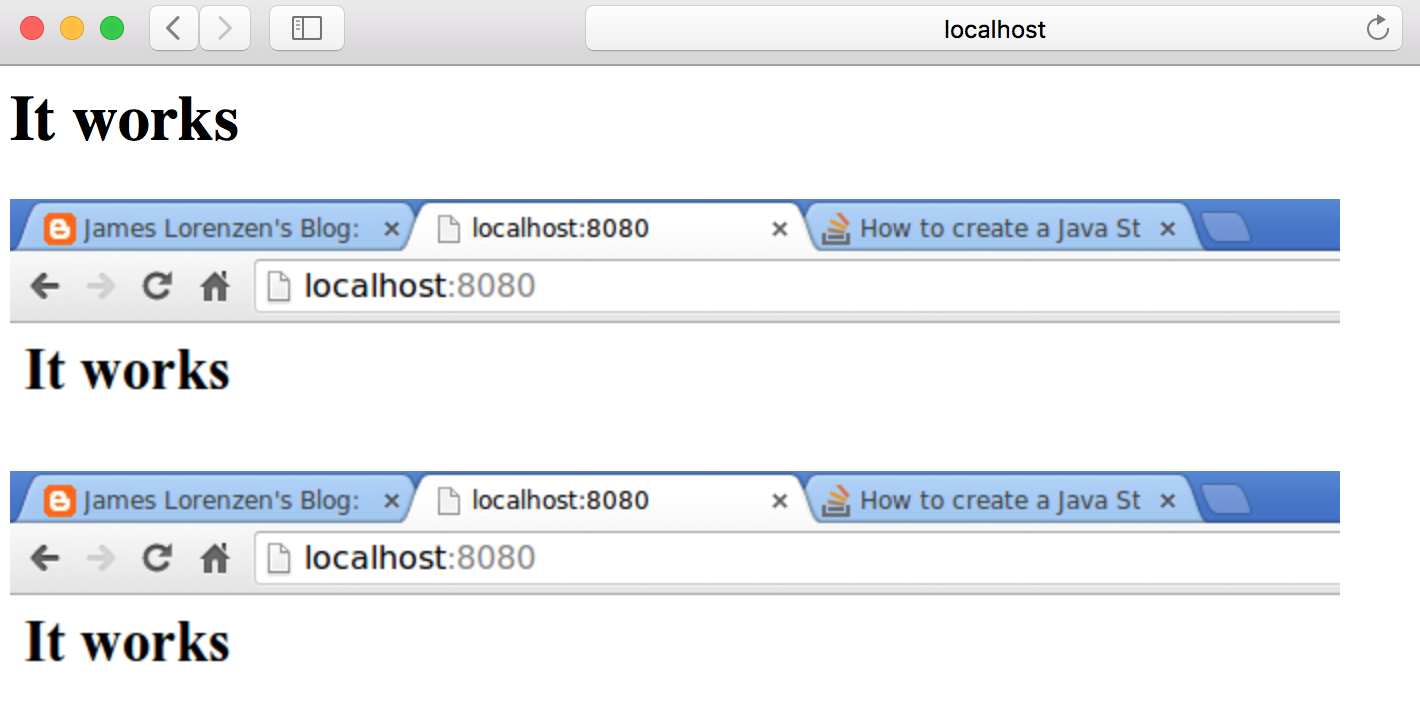
\includegraphics[scale=0.5]{output_clarification/TC1-1.png} 
\caption{Output for successfully starting server}
\label{TC1.1}
\end{figure}

\section{Use Case: Stop Server}

\subsection{Stopping Server}

An administrator should be able to stop the server by inputting "stop" into a running server's command line.

\subsubsection{Input}
\begin{itemize}
\item Web server is running on port 8080
\item Input "stop" into the server's command line window and press Enter
\item Open a web browser and navigate to "http://localhost:8080/"
\end{itemize}

\subsubsection{Output}
\begin{itemize}
\item A page with the header "Unable to connect" should appear in the web browser.
\end{itemize}


\subsection{Access log written to when server is stopped}

Make sure that an entry is written to the server's access log when an administrator manually stops the server.

\subsubsection{Input}
\begin{itemize}
\item Web server is running
\item Input "stop" into command line window and press Enter
\item Open sever access log in a text editor
\end{itemize}

\subsubsection{Output}
\begin{itemize}
\item The text "HTTP Server stopped" should be displayed on the last line of the access log.
\end{itemize}
\end{document}
